\part{La chaîne de traitement des actes princiers}

\chapter[Structuration des XML]{Structuration des XML à partir d'un script Python}

\vspace*{\stretch{1.3}} 
\par La conversion des documents ODT en XML avec \textit{Teinte} renvoie des documents TEI relativement structurés. Néanmoins, les balises ne sont pas conformes au format TEI. De plus, la structuration du document peut être encore améliorée, via la création d'attributs (caractéristiques d'une balise) par exemple. Le langage de programmation Python va permettre de lire les fichiers et d'intervenir dessus afin de parfaire l'organisation des actes. Python est un langage de programmation développé dans les années 1990 par le développeur Guido van Rossum. Il fournit une approche simple et efficace de la programmation orientée objet\footnote{La programmation orientée objet, ou programmation par objet, est une manière d'approcher la programmation via l'interaction de briques logicielles appelées objets. Les objets sont des structures de données avec le comportement associé, manipulés dans un programme. In : \cite{ProgrammationOrienteeObjet2021}.}, ce qui en fait un langage idéal pour les scripts et le développement d’applications dans de nombreux domaines\footnote{\og Le tutoriel Python \fg, in : \cite{ContenuDocumentationPython}.}.


\vspace*{\stretch{0.7}} 

\newpage 

\section[Extraction / Injection des données]{Extraction de données à partir des fichiers CSV et injections dans le XML
}
\label{III.5.1}

\par Une partie des données relatives aux actes de Charles I\up{er}, d’Agnès de Bourgogne et d’Anne Dauphine sont présentes dans un document CSV. Le format CSV, dont les valeurs sont séparées par des virgules, est le format le plus commun dans l'importation et l'exportation de feuilles de calculs et de bases de données\footnote{\og Lecture et écriture de fichiers CSV \fg, in : \cite{ContenuDocumentationPython}.}. Les CSV répertorient pour chaque duc et duchesse des informations essentielles sur les actes comme leur numéro, l'institution de conservation, le fond dont ils sont issus (identifiants), leur état, leur type diplomatique, l’année et la date de rédaction, les signataires, le lieu, les mentions de commandement, la langue de l'acte, et la présence ou non d’un sceau. 
\newline

\begin{figure}[ht]
    \centering
    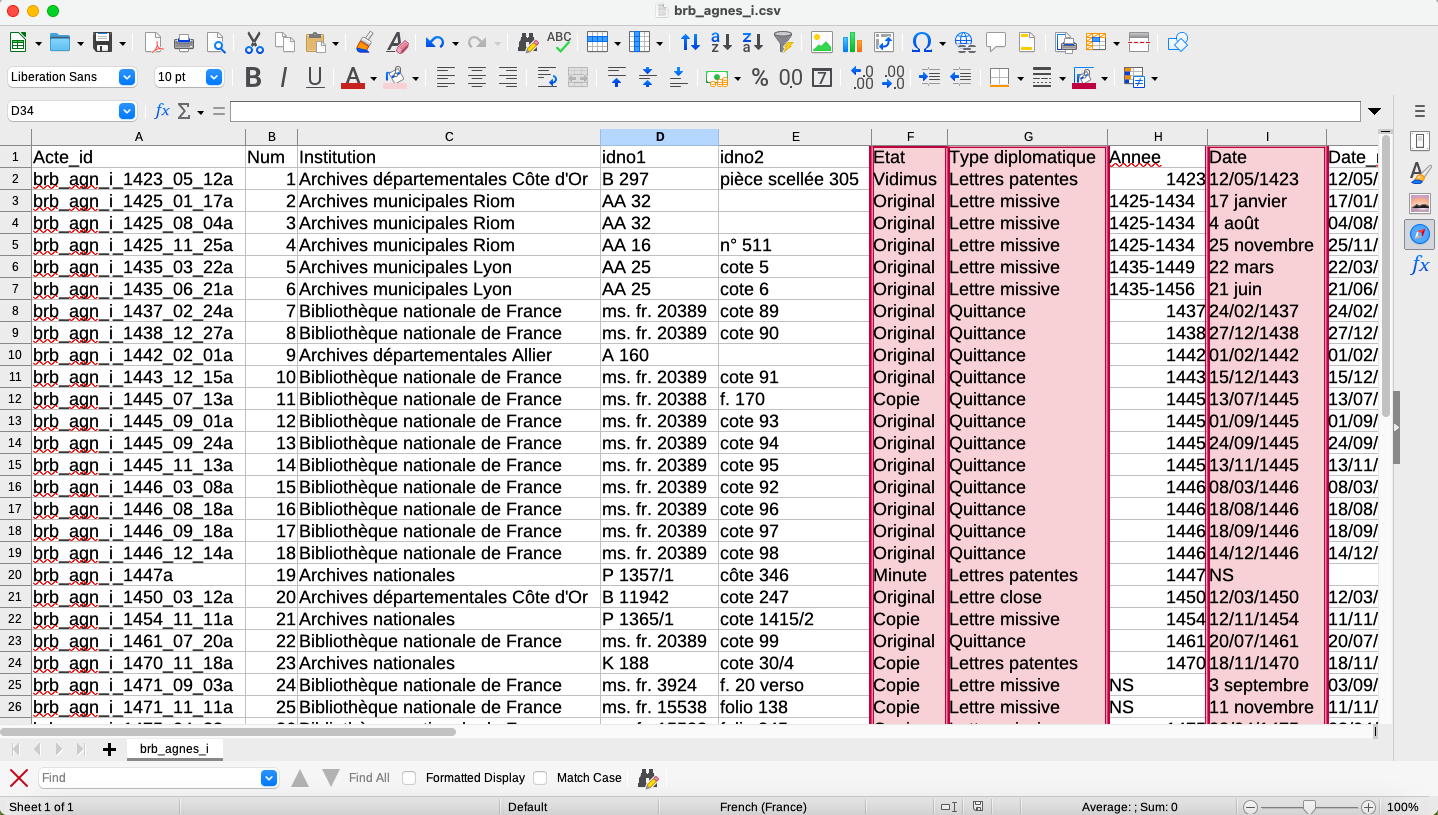
\includegraphics[scale=0.31]{front/images/csv_ad.png}
    \caption{CSV actes d'Agnès de Bourgogne.}
    \label{fig:csv}
\end{figure}

\par L’enjeu est d’extraire une partie des données des CSV : la date, l'état et le type diplomatique de chaque acte (valeurs surlignées en rose dans le tableur ci-dessus) afin de les ajouter comme attributs de la balise <div> du fichier XML créé pour chaque corpus. La date permettra également la création d'un attribut prenant la valeur d'un identifiant unique (@xml:id), pour chaque acte. Afin d'illustrer au mieux les modifications réalisées via Python, les figures qui suivent (figures 5.2 à 6.2) montrent les états successifs de l'acte daté du vingt-quatre février 1437 dans la chaîne de traitement des actes princiers.
\newpage 

\par Pour extraire les données en question, un script Python a été écrit\footnote{GitLab (py/add\_csv\_infos.py).}. 
\newline 
\par D'abord, une première fonction assure la lecture des fichiers XML à l'aide de la librairie \textit{BeautifulSoup}. Cette dernière permet l’extraction de données de fichiers HTML et XML. Afin de pouvoir l’utiliser correctement avec des fichiers XML, il est nécessaire d'importer le module \og bs4 \fg \space et d'installer le parseur \og lxml \fg \space conçu à cet effet. \textit{BeautifulSoup} fournit des moyens de navigation, de recherche et de modification de l’arbre XML. 
\newline 
\par Ensuite, une deuxième fonction constitue une liste avec les données du CSV qui seront transformées en attributs de la balise <div>. Elle nécessite d'importer le module \og csv \fg, qui permet de lire et d'écrire des données au format tabulaire CSV via les objets \og reader \fg \space et \og writer \fg. La fonction applique aux différents formats de dates un format standard afin de les agréger à un identifiant unique : xmlid. Deux modules sont importés pour assurer ces opérations : le module \og datetime \fg, qui fournit des classes pour manipuler les dates qui est complété par le module \og locale \fg \space qui prend en compte les spécificités de datation locales. La fonction comporte une première boucle qui itère sur chaque ligne du CSV. Si la valeur de la date est égale à \og Dep. \fg \space (deperditum), alors la date est manquante et un identifiant est créé. Si la date n’est pas \og Dep.\fg, une série de formats de date possibles est définie et stockée dans une liste. La fonction comprend une seconde boucle qui itère sur chaque format de date, les analyse, et en assure la conversion dans un format standard (YYYYMMDD). Elle permet également la création d'un identifiant unique pour chaque acte, à partir de cette date. La fonction retourne un dictionnaire composé des données extraites du CSV : date standard, état et type diplomatique, en préparation de leur injection aux fichiers XML. 
\newline 
\par Enfin, une troisième fonction injecte les données dans le XML. Après ouverture et lecture du fichier XML, elle itère sur toutes les balises <div> du <body> et leur ajoute les données extraites et modifiées comme attributs. L'attribut \og n \fg \space prend comme valeur la date au format standard, l'attribut \og xml:id \fg, l'identifiant unique créé à partir de cette date, l'attribut \og type \fg, l'état et l'attribut \og subtype \fg, le type diplomatique. Quelques opérations de mise en forme des documents ont été éfectuées, comme la suppression des lignes vides dans le nouveau document XML, via des expressions régulières, ce qui a nécessité l'importation du module \og re\fg. Les apostrophes odt sont également remplacées par des apostrophes standard et les balises <dateline> par des balises <head>. Les fichiers de sortie comportent les modifications réalisées par les trois fonctions. 
\newpage 

\begin{figure}[ht]
    \centering
    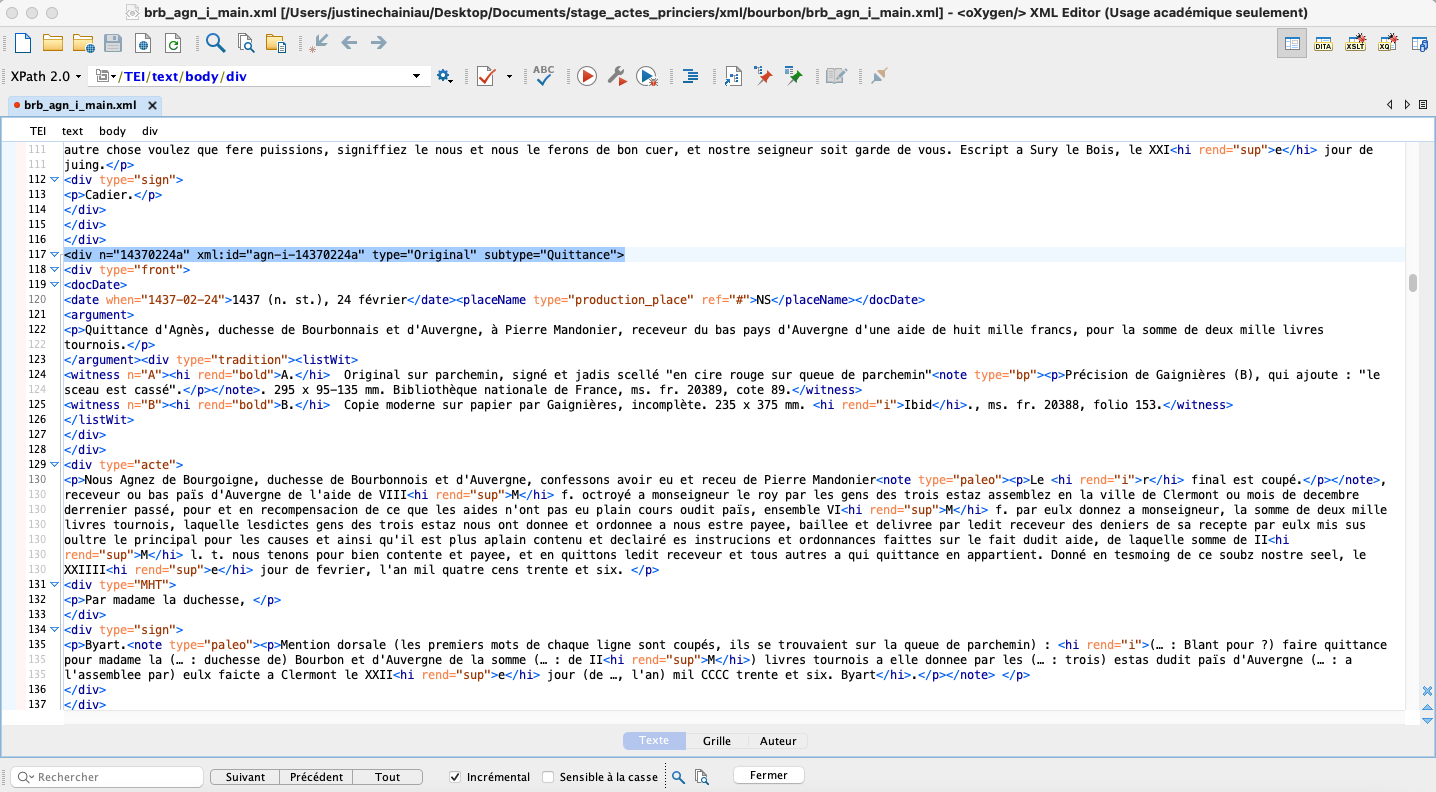
\includegraphics[scale=0.29]{front/images/injection.png}
    \caption{XML après injection des données avec Python.}
    \label{fig:injection}
\end{figure}

\par Les fonctions créées ont permis l'extraction de données de fichiers CSV et l'ajout de ces mêmes données dans du XML pour les actes d'Anne Dauphine, de Charles I\up{er} et d'Agnès de Bourgogne. Toutefois, les actes du corpus de Louis II ne sont pas répertoriés dans un CSV. Nous avons donc inversé la procédure afin d'en créer un.
\newline 

\par La fonction xml\_to\_csv créé un fichier CSV à partir de données extraites du fichier XML répertoriant les actes de Louis II\footnote{GitLab (py/div\_attributes.py).}. Une boucle itère sur chaque balise <div> et remplit, à partir d'information récupérées dans le XML, une liste. La fonction récupère le contenu de la balise <dateline>, qu'elle sépare en deux parties à partir d'une boucle. Si l'élément séparateur \og -\fg \space est présent dans le texte de la variable date, alors ce texte est divisé en deux parties qui forment deux items, afin de séparer la date de temps de la date de lieu. Sinon, le lieu n'est pas précisé et la mention \og NS\fg\footnote{NS : Non signalée.} \space est inscrite. La chaîne de caractère \og Louis II\fg \space est définie par défaut comme avant-dernier item de la liste, comme valeur de la colonne \og prince\fg. Pour la colonne \og signataire \fg, si la balise <signed> est présente dans les <div>, alors on complète la liste avec le contenu textuel de la balise <signed>, en omettant les diverses mentions \og (signé:)\fg. Autrement, la mention \og NS\fg \space lui est ajoutée. La mention \og fr\fg \space est répertoriée par défaut comme dernier item de la liste, comme valeur de la colonne \og langue\fg. En effet, seuls trois actes de Louis II sont en latin et ont été repérés préalablement : la colonne langue prend alors la valeur \og lat \fg \space pour les actes concernés\footnote{La Mure III, p.132 (10 juin 1370) - AD Allier, 1 G 3, fol. 1-6 (6 décembre 1386) \newline AN, P 1356\up{2}, c. 280 (18 septembre 1399).}. 
\newpage 

\par Ensuite, le fichier CSV est ouvert via la fonction \og open() \fg \space de Python, et les lignes sont remplies à partir des données stockées dans la liste. La ligne d'en-tête du fichier CSV est écrite à partir de la spécification du nom des colonnes : \og Date\fg, \og Lieu\fg, \og Prince\fg, \og Signataire\fg, \og Langue\fg, \og État\fg, \og Type diplomatique\fg. Néanmoins, ces deux dernières colonnes n'ont pu être complétées automatiquement, mais manuellement via le relevé de l'état de chaque acte et de son type diplomatique à partir du document ODT.
\newline 

\par La programmation en Python permet d'automatiser la manipulation des données, et ainsi de gagner du temps dans la chaîne de traitement. Toutefois, le processus se fonde sur les premiers corpus, qui disposent de fichiers CSV répertoriant les actes. En effet, la chaîne de traitement des actes princiers, telle qu'elle a été pensée par les ingénieurs du projet, nécessite qu'un certain nombre d'informations sur les actes soient présentes dans des fichiers CSV. Il faudra donc que les nouveaux corpus ajoutés au projet aient un CSV associé. Autrement, Python permet leur création via des fonctions, mais toute la procédure ne peut pas être automatisée, et toutes les colonnes remplies à partir de l'extraction de données. Des notions de diplomatique sont nécessaires afin de repérer, via la lecture de tous les actes, les états et les types diplomatiques, ce qui prend un certain temps, notamment dans le cas de corpus volumineux, comme ceux de Louis II et de Charles I\up{er}. Le projet \og Actes princiers \fg \space pourrait donc conseiller aux chercheurs qui élaborent des éditions diplomatiques de dresser en parallèle un tableur avec les différentes métadonnées. Les corpus disposent désormais tous d'un fichier CSV rempli, et les fichiers XML d'une balise <div> pourvue d'attributs qui contribuent à affiner l'organisation du document. Chaque acte est contenu dans une division (<div>) du document XML et identifié en tant que tel. Comme l'ensemble des balises n'est pas normalisé, les fonctions vont permettre de restructurer de manière automatique les documents XML.
\newpage 

\section[Restructuration des documents XML]{Restructuration des documents XML issus de la conversion}
\label{III.5.2}

\par Les documents XML obtenus en sortie, après intervention via un script Python, comportent désormais une balise <div> structurée. Toutefois, c'est l'ensemble du document qui nécessite d'être hiérarchisé. Il s'agit donc en utilisant Python de restructurer les documents selon le plan d'encodage ci-après, notamment en remplaçant les balises obtenues après conversion avec \textit{Teinte} en balises TEI afin d'obtenir un document XML valide. Comme l'indique le schéma ci-après, chaque acte doit être encodé dans une balise <div> comportant cinq autres balises <div>, qui représentent des subdivisions du corps du document\footnote{TEI Guidelines, <div>, en ligne : \url{https://tei-c.org/release/doc/tei-p5-doc/en/html/ref-div.html}.}. 
\newline 
\par La première d'entre elles comporte les éléments de datation et d'analyse. Les dates de temps et de lieu sont encodées dans deux balises distinctes. Le tableau de la tradition est ensuite structuré en une liste de témoins (<listWit>). Chaque témoin est encodé dans une balise dans laquelle sont imbriquées des balises pour le texte, l'institution de conservation et les identifiants (fonds et cote). Ensuite, une troisième <div> contient la teneur de l'acte dans une balise <p>, qui marque le début d'un paragraphe en prose\footnote{TEI Guidelines, <p>, en ligne : \url{https://tei-c.org/release/doc/tei-p5-doc/en/html/ref-p.html}.}. Si l'acte comporte un titre, il est encodé dans une balise <head>, qui marque l'en-tête (<head>Texte établi d'après A.</head>, <head>(Deperditum)</head>)\footnote{TEI Guidelines, <head>, en ligne : \url{https://tei-c.org/release/doc/tei-p5-doc/en/html/ref-head.html}.}. Pour finir, deux dernières balises <div> contiennent les mentions hors teneurs et les signataires dans des balises <p>. Ces opérations sont consignées dans des fichiers Python individuels pour chaque corpus : regex\_anne\_dauphine\footnote{GitLab (py/regex\_anne\_dauphine.ipynb).}, regex\_brb\_agnes\footnote{GitLab (py/regex\_brb\_agnes.ipynb).}, regex\_charles\footnote{Gitlab (py/regex\_charles\_i.ipynb).}, regex\_louis\footnote{GitLab (py/regex\_louis\_ii.ipynb).}. Il n'a pas été possible de traiter les quatre corpus à partir d'un seul script, car les documents ODT initiaux ne sont pas exactement structurés de la même manière. 

\begin{figure}[H]
    \centering
    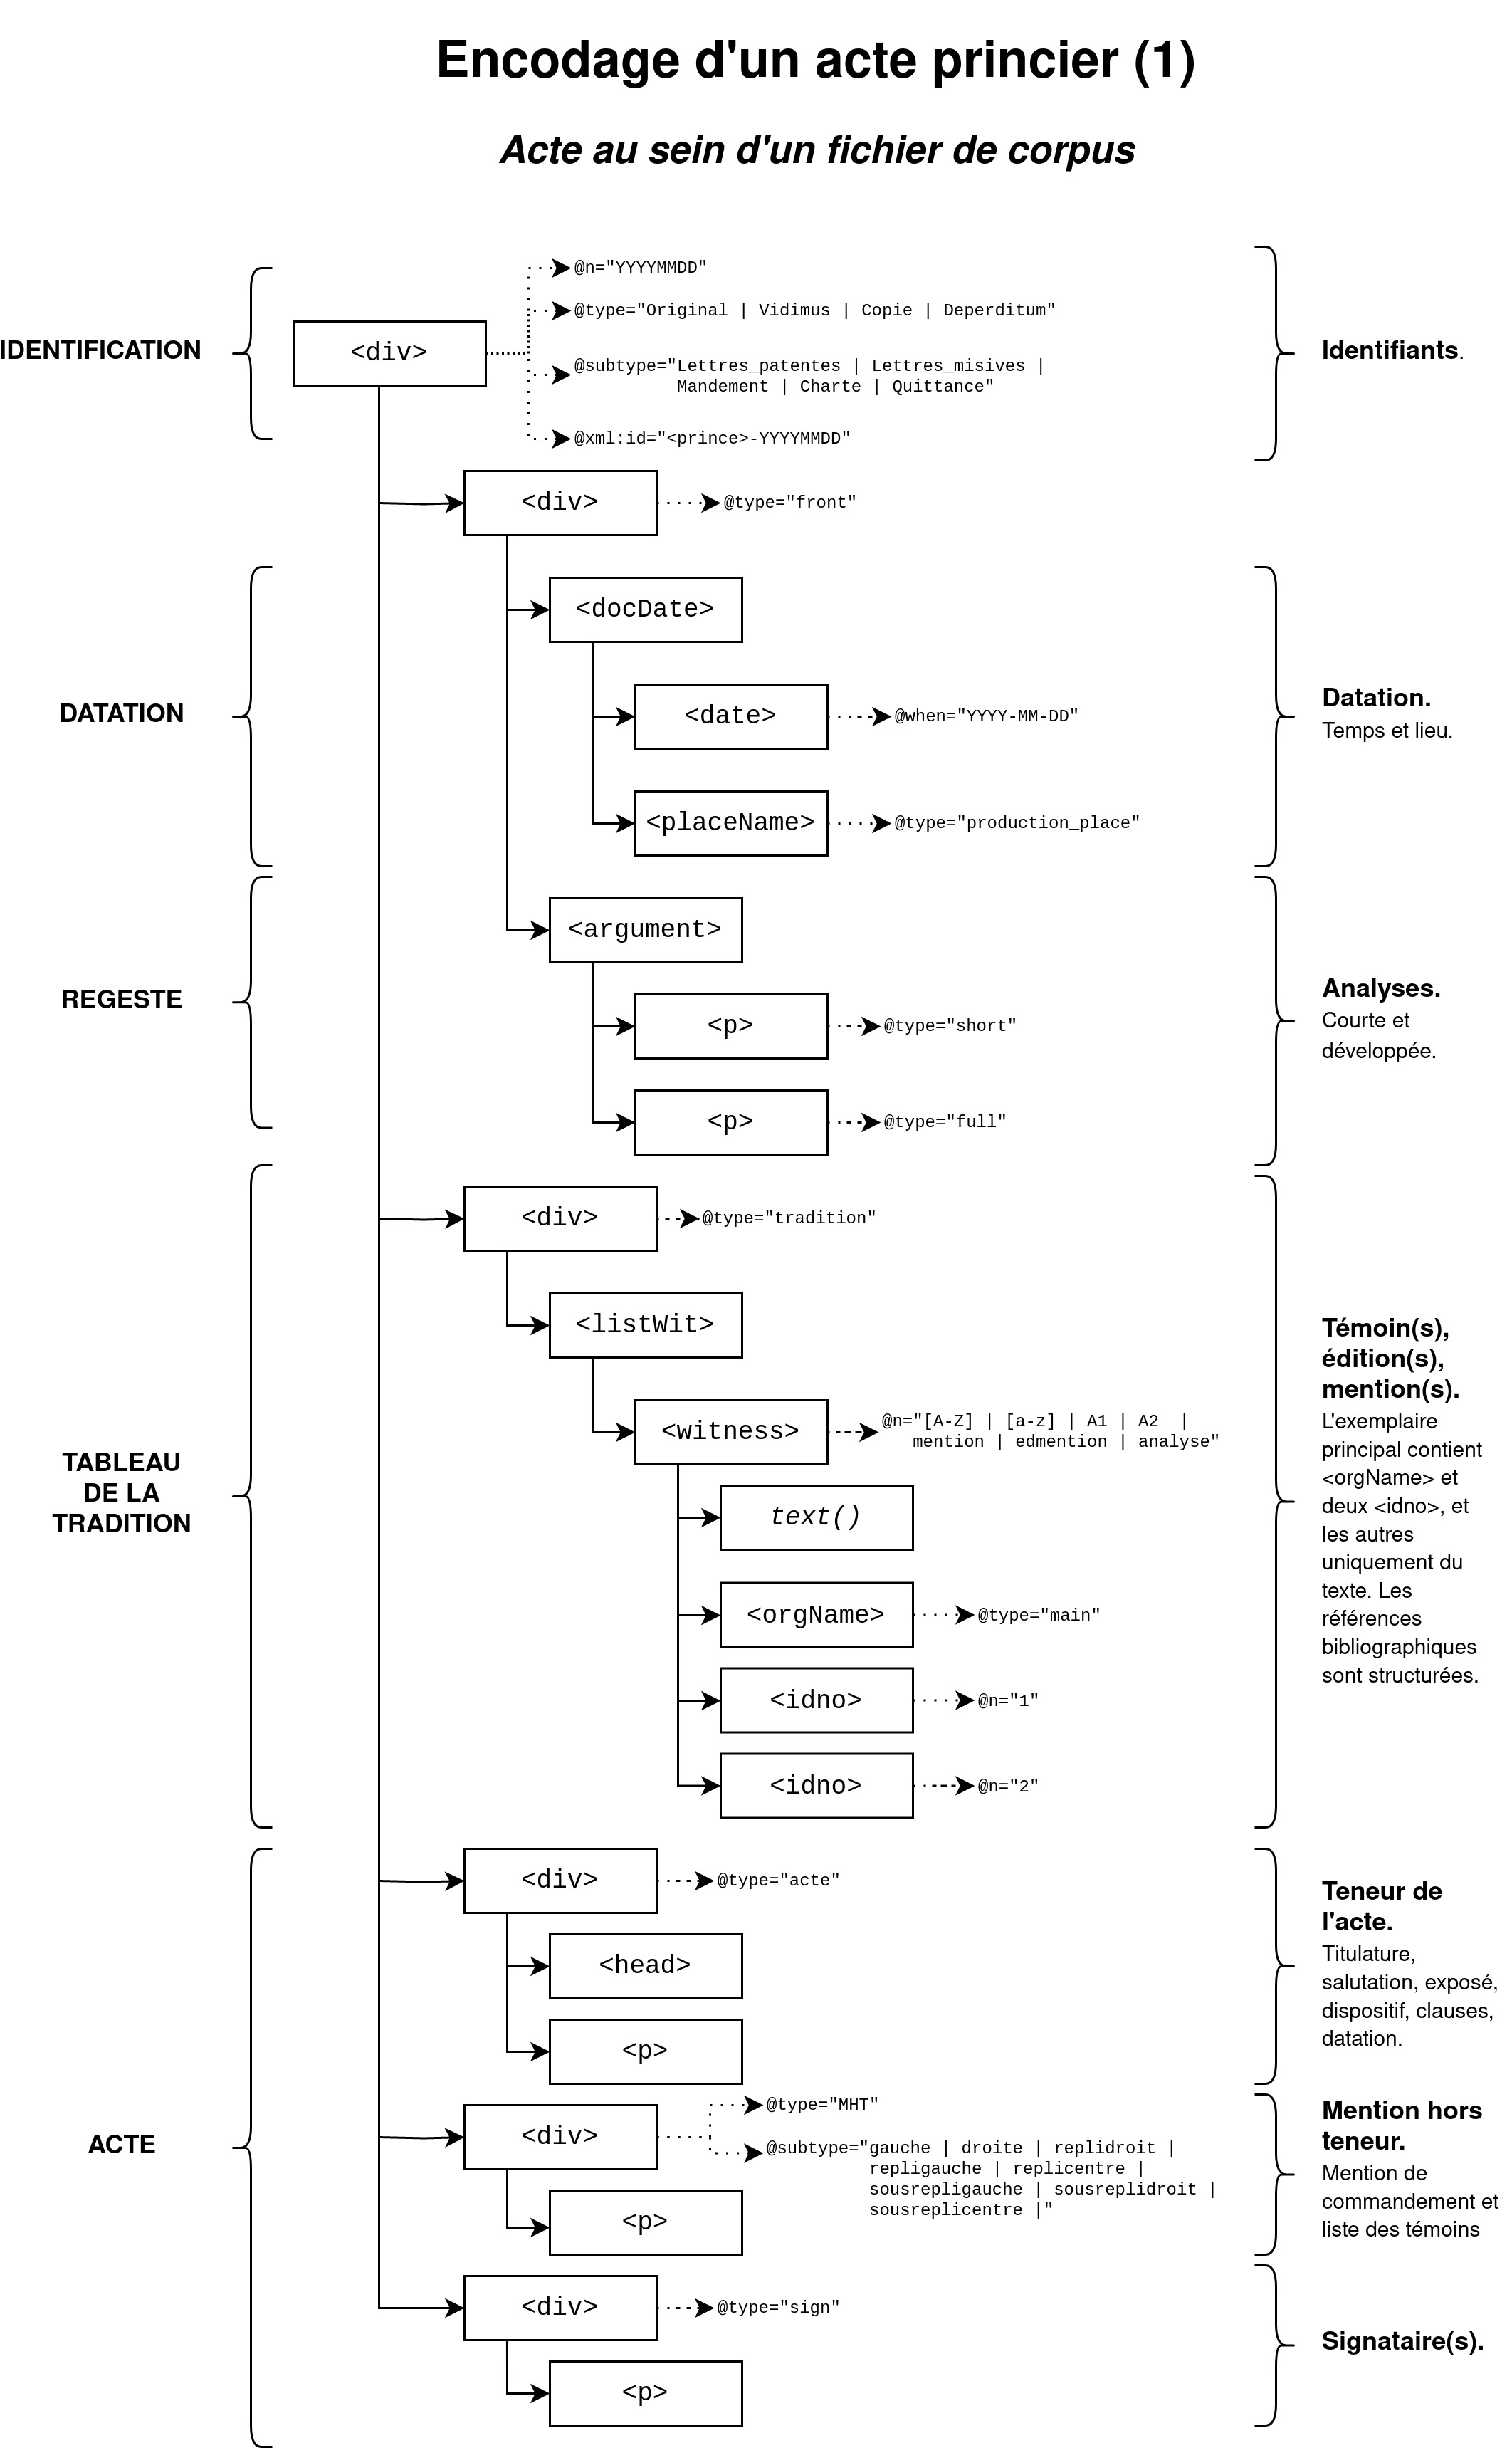
\includegraphics[scale=0.18]{front/images/encodage_actes_corpus.jpg}
    \caption{Schéma d'encodage des actes en XML. Source : Jean-Damien Généro.}
    \label{fig:encodage}
\end{figure}
\newpage 

\par D'abord, le script réalise des traitements automatiques via des regex pour améliorer la mise en forme des documents. Grâce à la fonction \og re.sub \fg, le code supprime un certain nombre d'éléments inutiles (balises inutiles, lignes vides) et substitue certaines balises afin d'obtenir une structuration plus fine. Ces opérations de substitution permettent l'insertion des principales <div> et éléments structurants comme <docDate>, spécifique pour la datation de documents\footnote{TEI Guidelines, <docDate>, en ligne : \url{https://tei-c.org/release/doc/tei-p5-doc/en/html/ref-docDate.html}.}, <argument>, cette dernière contenant une liste formelle ou une description en prose des sujets abordés dans une subdivision\footnote{TEI Guidelines, <argument>, en ligne : \url{https://tei-c.org/release/doc/tei-p5-doc/en/html/ref-argument.html}.} et <listWit>, qui énumère tous les témoins mentionnés par un appareil critique, éventuellement regroupés hiérarchiquement\footnote{TEI Guidelines, <listWit>, en ligne : \url{https://tei-c.org/release/doc/tei-p5-doc/en/html/ref-listWit.html}.}. Les illustrations à la page suivante donnent un aperçu des fichiers avant et après les interventions. Les premières balises structurantes sont ajoutées : <div type='front'> et <docDate> avec ses balises enfants. La balise <regeste> (qui peut être suvi d'une balise <hi>, marquant un mot ou une phrase comme graphiquement distinct du texte environnant\footnote{TEI Guidelines, <hi>, en ligne : \url{https://tei-c.org/release/doc/tei-p5-doc/en/html/ref-hi.html}.}) est substituée par la balise <argument> suivie d'une balise <p>. La fonction \og re.sub \fg permet la fermeture de certaines balises comme <p> et <argument> et d'intégrer les balises ouvrantes suivantes : <div type='tradition'> et <listWit>. Cette opération est répétée afin de fermer la balise </listWit> et d'ajouter les suivantes : </div>, </div>, <div type="acte"> et <p>. Les cas particuliers des actes commençant par un titre ou comportant la mention \textit{deperditum} sont réglés par des regex. Puis, la balise <div type="acte"> est fermée, ainsi que celle du dernier acte, dont le traitement n'est pas automatique. Le <tableautradition> est suppléé par la balise <witness> contenant la description précise d’un seul témoin\footnote{TEI Guidelines, <witness>, en ligne : \url{https://tei-c.org/release/doc/tei-p5-doc/en/html/ref-witness.html}.}, avec ses attributs et suivi du n° d'exemplaire. Les spécifications <analyse>, <edmention> et <mention> sont toutes remplacées par la balise <witness>, dont la balise fermante est ajoutée. Les dernières balises <mentioncommandement> et <signed> sont changées en balises <div> disposant respectivement d'attributs \og MHT \fg \space et \og sign \fg. 
\newpage

\begin{figure}[H]
    \centering
    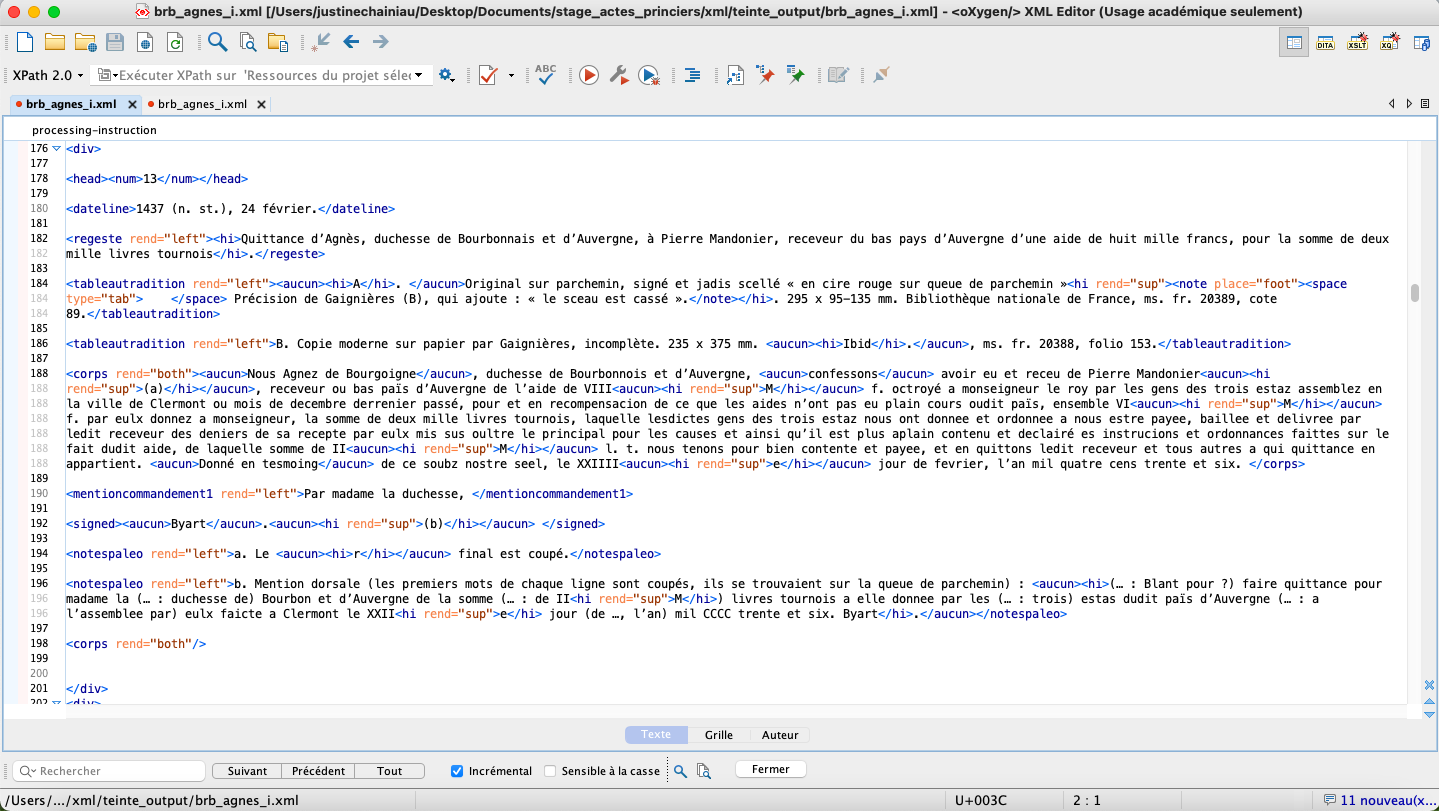
\includegraphics[scale=0.3]{front/images/teinte_agnes.png}
    \caption{Encodage de l'acte daté du 24 février 1437 avant intervention.}
    \label{fig:encodage_avant}
\end{figure}

\begin{figure}[H]
    \centering
    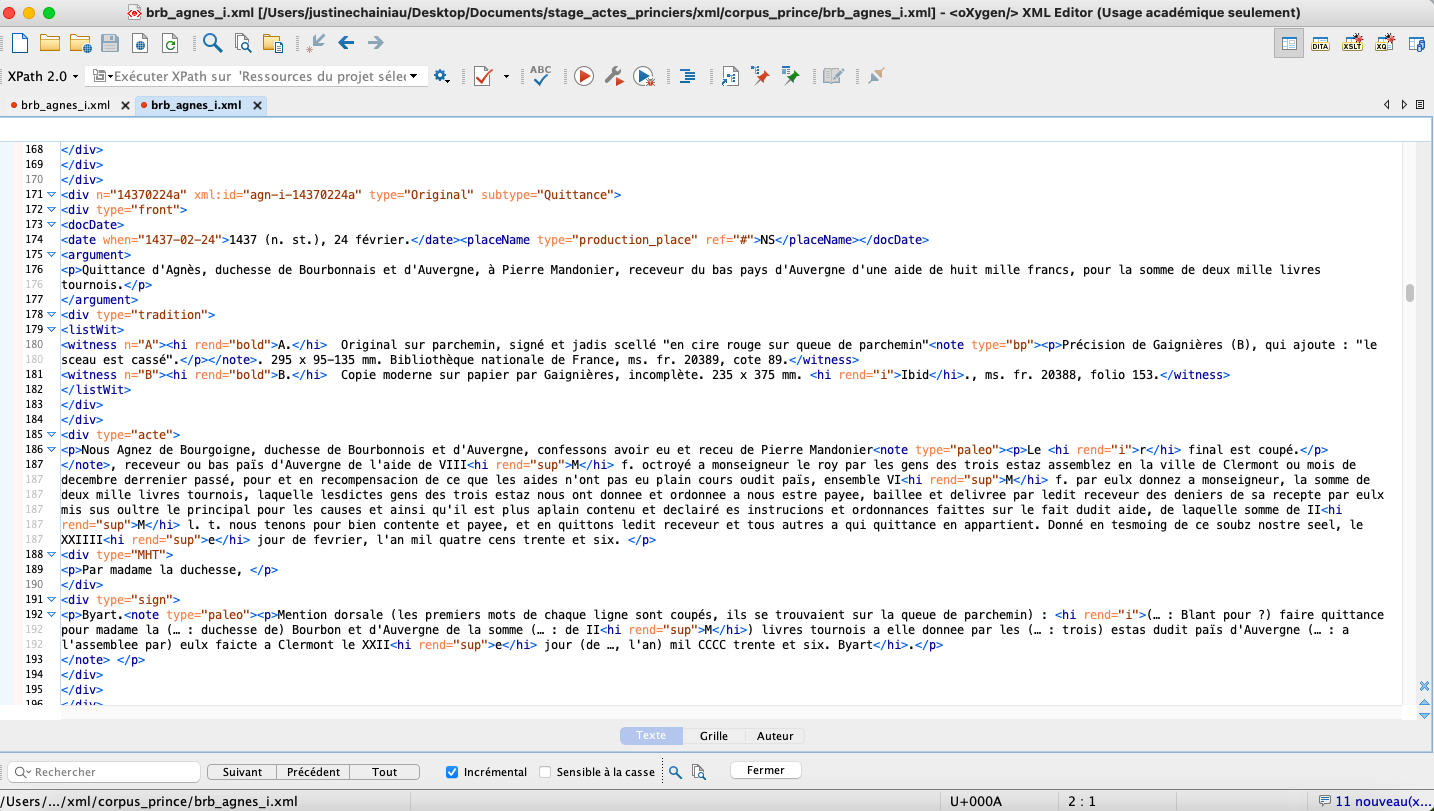
\includegraphics[scale=0.3]{front/images/restruct_agnes.png}
    \caption{Encodage de l'acte daté du 24 février 1437 après intervention.}
    \label{fig:encodage_après}
\end{figure}
\newpage 

\par Ensuite, le script réalise des traitements semi-automatiques. En raison des disparités entre les quatre corpus, toutes les opérations ne peuvent pas être réalisées de manière automatique. De plus, les regex de l'étape précédente n'ont pas toujours fonctionné. En effet, la chaîne de traitement bute sur des erreurs de mise en forme des éditeurs. L'option de validation d'Oxygen nous a permis de repérer les problèmes d'encodage et de les corriger un à un dans le script via une regex dédiée. Ces irrégularités sont pour une grande partie liées à la balise <hi> qui est parfois présente en trop ou manquante. De plus, les mentions \og (Signé :) \fg \space comportent des fautes d'encodage et n'ont, par conséquent, pas toujours été supprimées par le script. Les erreurs spécifiques à chaque corpus sont traitées individuellement. Toutes les corrections sont stockées dans un dictionnaire qui se substituera aux valeurs précédentes. Les dernières erreurs concernent la mise en forme des notes de bas de page et des notes paléographiques. Le nombre d'appels de note diffère du nombre de notes. Cela est généralement dû aux manquements dans le stylage effectué précédemment, ou à leur présence en double. Après quelques corrections de mise en forme : traitement des espaces insécables, des guillemets, des balises <hi> sans attributs, le fichier est écrit dans un document. Le parseur lxml repère les fautes de syntaxe et traite les caractères non valides. Les éléments HTML, s'il y en a, sont retirés et les octets XML sont décodés en une chaîne de caractères afin d'inscrire le contenu XML dans un fichier.
\newline 

\par Enfin, en fonction des erreurs relevées, des corrections sont effectuées avec lxml. L'objectif principal est la structuration des dates en un bloc. Pour cela, il s'agit d'ajouter à la nouvelle balise <date> un attribut \og when \fg \space avec la date au format standard YYYYMMDD, ou YYYYMM ou YYYY. Puis, les notes paléographiques sont alignées sur leurs appels de note. La dernière correction concerne les attributs \og xml:id \fg \space et \og n \fg. En effet, lorsque deux actes sont datés du même jour, ils ont le même identifiant, or ces derniers doivent être uniques dans un document XML.
\newline 

\par La suppression et la substitution de balises via une fonction Python a permis de structurer très finement les documents avec des balises XML imbriquées et dotées d'attributs. Toutefois, certaines opérations se sont montrées plus complexes, comme la hiérarchisation du tableau de la tradition, qui n'est pas aussi fine que sur le schéma d'encodage établi en amont\footnote{Figure 5.3 – Schéma d’encodage des actes en XML.}. En effet, la balise <witness> ne comporte pas les balises <text>, <orgName> et <idno>. Même si le document obtenu en sortie ne respecte pas exactement le schéma théorique, la plupart des balises ont été transformées. Les fichiers XML bénéficient désormais d'une structure robuste permettant leur division en fichiers XML individuels pour chaque acte.
\newpage 


\section[Séparation des fichiers]{Séparation des fichiers XML de corpus en fichiers XML d’actes}
\label{III.5.3}

\par L'objectif est de transformer le fichier XML contenant l'ensemble des actes d'un prince obtenu après interventions en autant de fichiers XML qu'il y a d'actes. Une fonction Python : split\_corpus\footnote{GitLab (py/split\_corpus.ipynb).} est utilisée pour réaliser cette opération. Cette fois-ci, une seule fonction est adaptable pour les quatre corpus, dans la mesure où ils ont été normalisés en amont. La première étape est la création d'un fichier XML par acte. Cela passe par la récupération des <div> des actes en itérant sur chaque balise. Les données sont alors stockées dans une liste, qui, couplée au canevas TEI suivant, permet la constitution du fichier.
\newline 

\textbf{CANEVAS TEI} \newline 
<TEI xmlns="http://www.tei-c.org/ns/1.0"> \newline 
<teiHeader> \newline 
<fileDesc> \newline 
<titleStmt> \newline 
<title level="s">Actes princiers</title> \newline 
<title level="m">+++TITLE+++</title> \newline 
<title level="a"></title> \newline 
<respStmt> \newline 
<resp>transcribed by</resp> \newline 
<name>+++TRANSCRIPTEUR+++</name> \newline 
</respStmt> \newline 
</titleStmt> \newline 
<editionStmt> \newline 
<edition>Acte édité dans le cadre du programme Actes princiers.</edition> \newline 
<respStmt> \newline 
<resp>direction scientifique</resp> \newline 
<name>Olivier Mattéoni</name> \newline 
</respStmt> \newline 
<respStmt> \newline 
<resp>direction technique</resp> \newline 
<name>Jean-Damien Généro</name> \newline 
</respStmt> \newline 
<respStmt> \newline 
<resp>direction technique</resp> \newline 
<name>Nicolas Perreaux</name> \newline 
</respStmt> \newline 
<respStmt> \newline 
<resp>stagiaire de l'École nationale des chartes</resp> \newline 
<name>Justine Chainiau</name> \newline 
</respStmt> \newline 
</editionStmt> \newline 
<publicationStmt> \newline 
<publisher>Laboratoire de Médiévistique occidentale de Paris (UMR 8589), Centre de recherches historiques (UMR 8558)</publisher> \newline 
<authority>Olivier Mattéoni</authority> \newline 
<date when="2023">2023</date> \newline 
<availability><licence source="https://github.com/etalab/licence-ouverte/blob/master/open-licence.md">Distributed under an Open License 2.0</licence></availability> \newline 
</publicationStmt> \newline 
<sourceDesc> \newline 
<msDesc> \newline 
<msIdentifier> \newline 
<repository></repository> \newline 
</msIdentifier> \newline 
<msContents> \newline 
<msItem> \newline 
<docDate></docDate> \newline 
</msItem> \newline 
</msContents> \newline 
</msDesc> \newline 
<listPerson> \newline 
<listPerson type="prince"/> \newline 
<listPerson type="signatory"/> \newline 
</listPerson> \newline 
</sourceDesc> \newline 
</fileDesc> \newline 
<profileDesc> \newline 
<abstract> 
<p></p> 
</abstract> \newline 
</profileDesc> \newline 
</teiHeader> \newline 
<text> \newline 
<body> \newline 
</body> \newline 
</text>
</TEI> \newline 

\par La fonction complète le TEI Header ci-dessus avec une partie des données présente dans le CSV. Le nom du prince à l'origine de l'acte est ajouté à la balise <listPerson type="prince">, ceux des signataires dans la balise <listPerson type="signatory">. L'institution de conservation, le fonds et la cote sont également extraits des colonnes du CSV. Les éléments HTML sont encore une fois retirés, et les octets XML décodés en une chaîne de caractère afin d'inscrire le contenu XML dans un fichier. 
\newline 

\par L'activation des fonctions passe par la création d'un dictionnaire contenant en clef l'identifiant de la maison et celui du prince, et en valeur une liste avec : le chemin vers le fichier XML du prince depuis le dossier /py, le nom du CSV du prince, le nom du dossier où seront enregistrés les XML des actes, le titre du corpus et le nom du transcripteur. La fonction est activée via une itération sur le dictionnaire et permet la transformation des fichiers. Le fichier ci-après montre le résultat obtenu après division du fichier contenant tous les actes du corpus. 
\newline 

\begin{figure}[H]
    \centering
    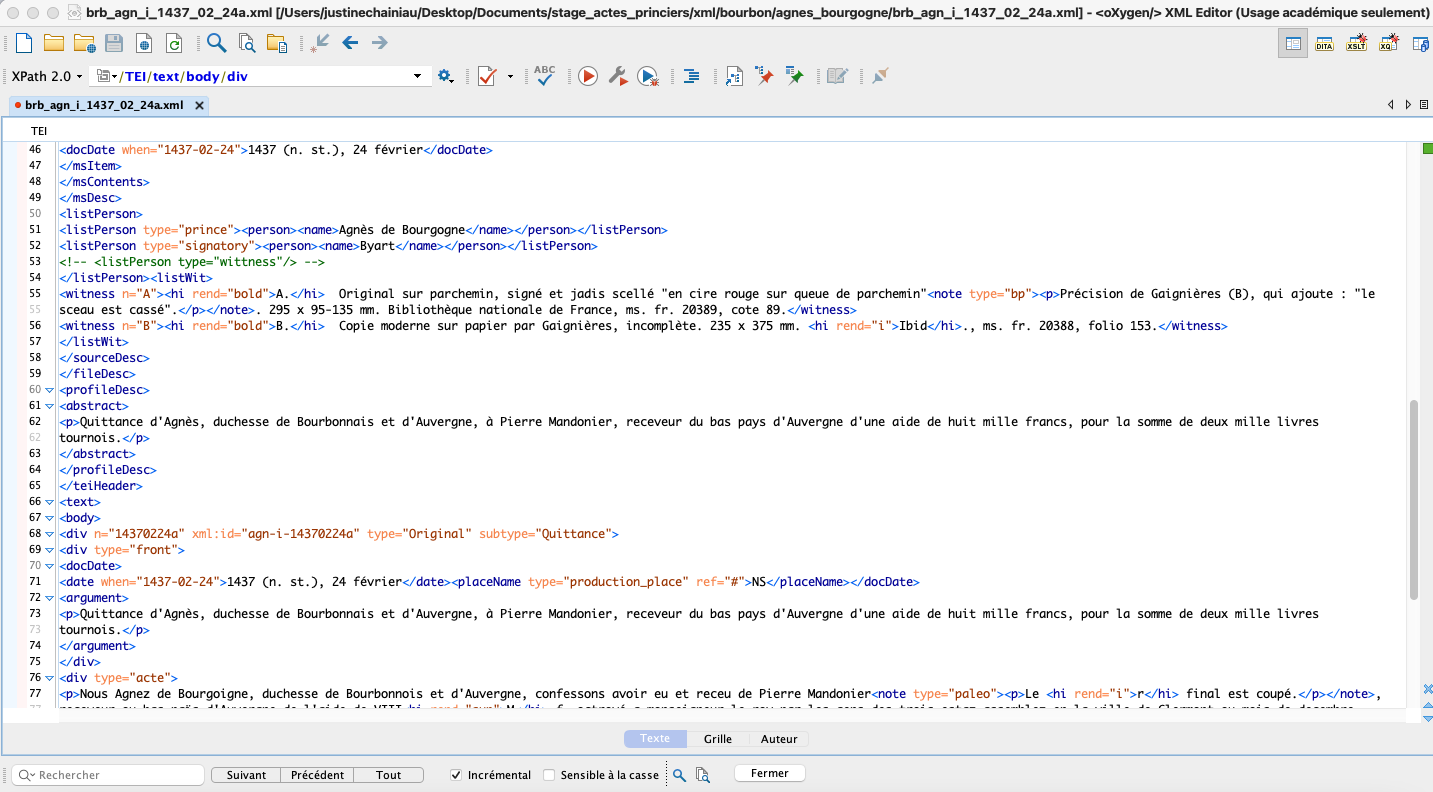
\includegraphics[scale=0.31]{front/images/fichier_indiv.png}
    \caption{Fichier XML de l'acte daté du 24 février 1437.}
    \label{fig:fichier_indiv}
\end{figure}
\newpage 

\par Les fichiers individuels sont pourvus d'un TEI Header complété d'informations générales, ajoutées à tous les actes. Le <Filedesc> comporte la description bibliographique du document. La balise <titleStmt> comprend plusieurs balises imbriquées correspondant à plusieurs niveaux de titre. Ensuite, la balise <editionStmt> présente le projet d'édition ainsi que les personnes en charge de celui-ci. Les indications sur la diffusion du fichier numérique et ses droits d’utilisation (licence) sont dans le <publicationStmt>. Les données individuelles, propres à chaque fichier et extraites du CSV sont placées dans le <sourceDesc>, qui décrit le document source. Cette balise contient les éléments d'identification, de conservation, de datation de l'acte ainsi que la liste des personnes concernées (signataires et prince à l'origine de l'acte) et le tableau de la tradition. Ces éléments sont suivis du <profileDesc>, qui fournit une description détaillée des aspects non bibliographiques, des informations contextuelles, notamment via l'analyse de l'acte en question. Le TEI Header est suivi de l'édition encodée pour chaque acte. 
\newline 

\par L'utilisation de Python via des fonctions a permis de manipuler les données et ainsi d'améliorer la structuration des documents. D'abord via l'extraction de données dans d'autres documents qui n'étaient pas au format XML (CSV), puis via la substitution des balises initiales issues de la conversion en des balises TEI standard, enfin par la séparation des fichiers XML obtenus en fichiers individuels. Ces étapes ont répondu à l'objectif fixé initialement, à savoir l'encodage des éditions des actes selon le schéma établi en amont, et sont préalables à la mise en ligne des documents. 

\newpage
\thispagestyle{empty}
\mbox{}
\newpage

\chapter{Préparation à la mise en ligne des données}

\vspace*{\stretch{1.3}} 
\par Ce chapitre présente les dernières étapes de la chaîne de traitement, préalables à la mise en ligne des données. Avant cette dernière, les fichiers XML sont uniformisés, et bénéficient de corrections individuelles, souvent manuelles, puis sont transformés en LaTeX via XSLT et compilés en PDF. L'objectif est de pouvoir relire les actes et d'y repérer les erreurs, sans avoir à ouvrir un à un les documents XML. LaTeX est un langage et un système de composition de documents largement employé par la communauté scientifique qui met l'accent sur la structure et le contenu du texte, en codant la mise en page des documents\footnote{\cite{LaTeXDMS}.}. 
\vspace*{\stretch{0.7}} 
\newpage 

\section[Transformation et compilation des fichiers]{Transformation du XML en LaTeX et compilation en PDF}
\label{III.6.1}

\par Le langage LaTeX sépare le fond de la forme en définissant sémantiquement le contenu via des commandes. Il permet une gestion automatique du référencement (gestion des différentes parties d'un ouvrage : chapitres, citations, notes ...) et une typographie de qualité\footnote{\cite{LaTeXDMS}.}. Pour l'édition d'actes, les différentes parties sont mises en valeur. Chaque acte édité est inséré dans un groupe. La date fait office de titre en gras, l'analyse figure ensuite en italique, puis viennent le tableau de la tradition et le contenu textuel. Toutes ces parties sont séparées par des commandes de mise en forme (espaces, sauts de lignes ...). 
\newline 

\begin{figure}[H]
    \centering
    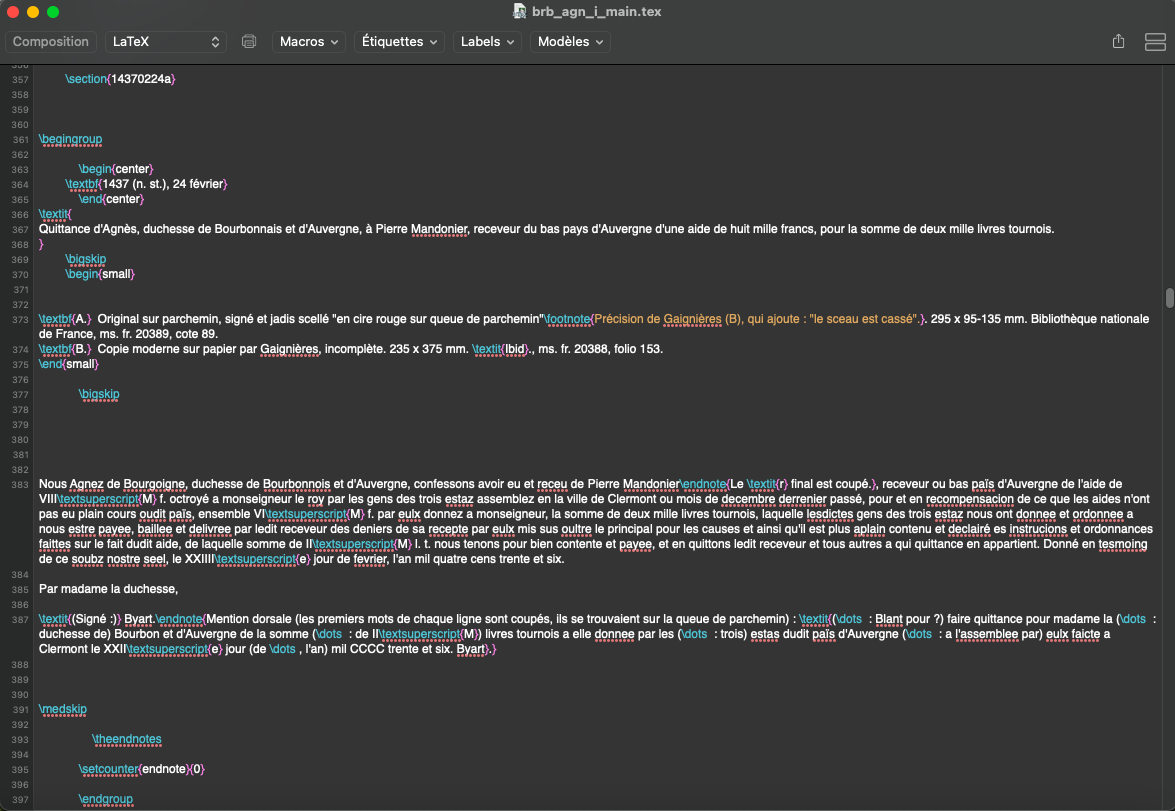
\includegraphics[scale=0.39]{front/images/latex.png}
    \caption{Fichier tex des actes d'Agnès de Bourgogne.}
    \label{fig:latex_agnes_db}
\end{figure}

\newpage 

\par L'objectif est d'assembler à nouveau tous les fichiers XML individuels obtenus pour chaque acte dans un seul fichier XML. La transformation de ce fichier en LaTeX permettra sa compilation et donc sa conversion et lecture au format PDF. Cela est réalisé grâce à une fonction Python\footnote{GitLab (py/compilation\_latex.ipynb).} qui transforme la langage XML en langage tex via XSLT. XSLT est le langage conçu pour transformer des documents XML en d’autres documents selon les spécifications XSL. XSL (eXtensible Stylesheet Language) désigne les spécifications pour écrire des feuilles de style, soit de quelle manière doivent être transformés les documents XML. Une fois le document correctement codé, une étape de compilation permet d'en produire un rendu final, ici un PDF mis en page. 

\begin{figure}[H]
    \centering
    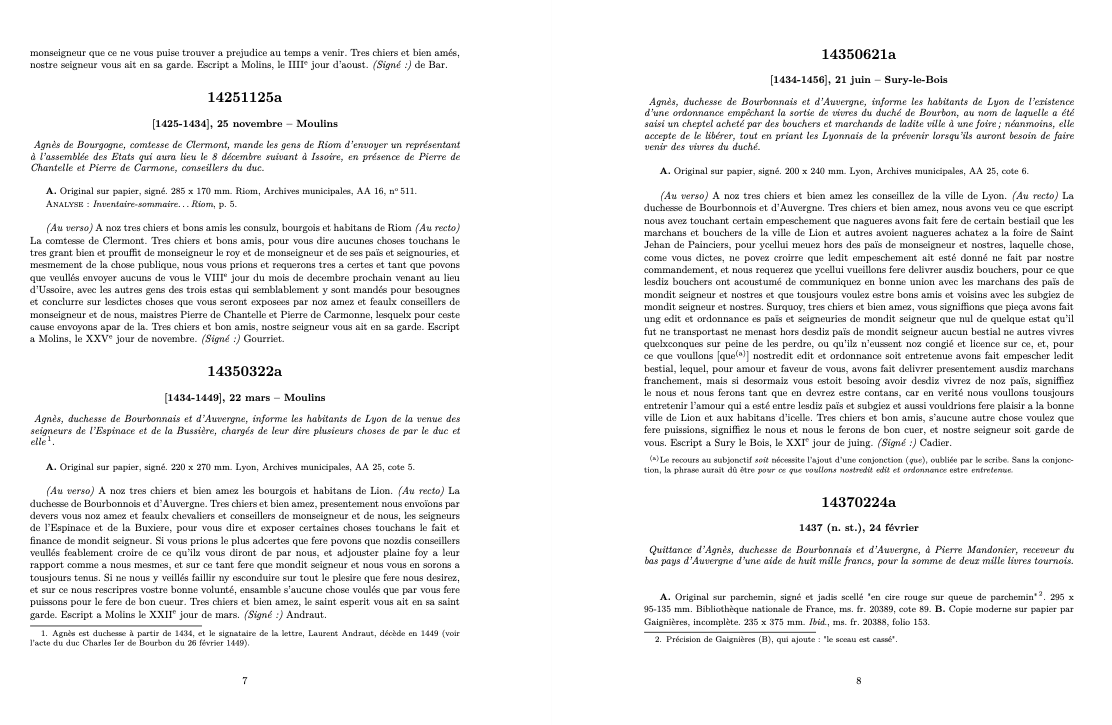
\includegraphics[scale=0.41]{front/images/pdf_compile_ab.png}
    \caption{Fichier PDF des actes d'Agnès de Bourgogne issu de la compilation du fichier tex.}
    \label{fig:pdf_conpile}
\end{figure} 

\par Les éditions une fois compilées en PDF rassemblent l'intégralité des actes pour chaque duc et duchesse. Chaque acte se distingue par son identifiant unique en gras et dans une taille plus importante. Ensuite, les dates de temps et de lieux apparaissent également en gras, séparées par une virgule. L'analyse en italique précède le tableau de la tradition, dont la numérotation des mentions est indiquée en gras. Puis vient le texte de l'acte, suivi des mentions hors teneurs indentées et du nom des signataires précédé de la mention \og (Signé:)\fg. Selon les cas, les notes paléographiques sont situées après le texte, en toutes petites capitales, alors que les notes de bas de page apparaissent en fin de page.  

\par La conversion du XML en tex permet la compilation puis une lecture agréable des éditions en PDF. L'ensemble de ces langages sont privilégiés par les travaux de recherche dans la mesure où ils assurent l'intégrité des données dans le temps. LaTeX est un logiciel libre, gratuit, multiplateforme et donc compatible avec différents systèmes d'exploitation et sans risque d'obsolescence. De plus, le programme est robuste, stable, compilé puisqu'il se met à jour lors de chaque compilation\footnote{\cite{LaTeX}.}. L'ensemble des technologies utilisées pour la transformation des documents permet donc la génération d'édition standard et mises en forme selon les \textit{Conseil pour l'édition de texte médiévaux} de l'École Nationale des Chartes\footnote{\cite{guyotjeanninConseilsPourEdition2009} \newline \cite{guyotjeanninConseilsPourEdition2014}.}. Toutefois, certaines erreurs de mise en page ont été repérées au sein des PDF. 
\newpage 

\section{Uniformisation des fichiers XML}

\par Après relecture des documents PDF générés, des anomalies figurent dans l'édition des actes\footnote{GitLab (medieval-acts/princely-acts/stage\_actes\_princiers\#7).}. Elles sont visibles et repérables au sein des PDF. Une fois identifiées, nous avons constaté qu'elles étaient souvent dues à des erreurs dans l'encodage des documents XML et à des erreurs de mise en forme. Les corrections sont effectuées au sein des fichiers individuels dans la mesure où les fichiers regroupant tous les actes pour chaque duc et duchesse, permettant par la suite la transformation en tex puis la compilation en PDF, sont générés à partir des fichiers individuels. Le mode projet d'Oxygen (l'éditeur XML) a permis de corriger ces écarts sur l'ensemble des fichiers individuels pour chaque prince, et même sur l'ensemble des quatre corpus, dans la mesure où il permet de naviguer dans l'arborescence du dossier XML du projet. 
\newline 

\par Les erreurs individuelles, propres à chaque corpus, ont été révisées en première intention. Le corpus de Louis II présente le plus d'anomalies.
L'une d'entre elles a été réglée directement via le script Python. Il s'agit de la suppression de la commande \og textsuperscriter \fg \space qui apparaissait dans la date de temps des actes datés du premier jour d'un mois. Le reste a été corrigé directement dans les fichiers XML. Premièrement, des regex ont été utilisées pour pallier les problèmes d'encodage. Les balises <hi> ne sont pas toujours encodées correctement. Certaines ne contiennent que des points ou une parenthèse. La mention \og signé \fg \space n'est pas continuellement insérée dans des balises <hi>, et est parfois fractionné. De plus, elle est parfois présente en double dans le document PDF, et n'est pas toujours indentée. Une centaine d'actes sont affectés par ces doubles mentions. En effet, elles sont ajoutées par XSLT, d'où la nécessité de les supprimer directement des XML via une regex. Les expressions régulières ont permis de remplacer les éléments (balises et leur contenu) incomplets par des éléments normalisés. Par ailleurs, une partie des défauts relevés dans les PDF proviennent des CSV. En effet, c'est par la ponction d'informations dans ces fichiers et leur ajout au XML que des éléments déficients se sont retrouvés par la suite dans le PDF. L'attribut de la balise <subtype> \og Traité-Accord \fg \space qui indique le type diplomatique de l'acte et atteste d'un accord passé entre plusieurs princes correspond en fait à des lettres patentes\footnote{AN, P 1357\up{2}, n°425 (13 août 1377). - AN, P 1370\up{2}, c. 1920 (21 avril 1386).}. Cet élément n'avait pas été revu dans le CSV des actes de Louis II et a ainsi été ajouté comme attribut de la première balise <div> dans les fichiers XML. À l'instar des XML, les fichiers CSV ont également bénéficié d'une révision, en supprimant et en remplaçant les mentions défaillantes par les mentions correctes via des regex. 
\newpage 

\par Deuxièmement, il est possible de corriger certains éléments en utilisant le Xpath, le chemin qui permet de naviguer au sein de l'arbre XML. Des points d’interrogations, qui marquaient des incertitudes sur les types diplomatiques dans les CSV, ont été relevés au sein des balises <subtype> et <type>, puis éliminés. Troisièmement, les erreurs singulières ont été corrigées manuellement. C'est le cas d'une date de temps qui était doublée (acte daté du vingt-deux septembre puis signé le vingt-sept septembre) et encodée dans la date de lieu\footnote{AN, P 1357\up{2}, n°442 (22 et 27 septembre 1399).}. Une référence a aussi été trouvée dans une date de lieu. Le corpus d'Anne Dauphine ne comporte quant à lui qu'une date de temps encodée dans une date de lieu, qui a également été retirée manuellement. 
\newline 

\par Le corpus de Charles I\up{er} comporte une erreur majeure due au remplissage du CSV, qu'il est possible de corriger via une regex. Le type diplomatique n'est pas normalisé : on retrouve la mention \og dep \fg \space au lieu de \og deperditum \fg. Les expressions régulières ont permis le remplacement instantané des cent trente-trois occurrences à la fois dans le CSV et dans les fichiers XML. Le corpus d'Agnès de Bourgogne n'est pas non plus exempt d'erreurs d'encodage. En effet, la plupart des dates de lieu des actes sont encodées dans la balise <date>. Ainsi, seules des mentions \og NS \fg \space sont encodées dans la balise <placeName>. En conséquence, lors de la transformation, les mentions \og NS \fg \space ne sont pas interprétées et la date de temps et la date de lieux ne sont donc pas séparées par des tirets dans le PDF puisqu'elles sont encodées dans la même balise. Cela a été corrigé manuellement dans la mesure où les actes concernés n'étaient pas trop nombreux.
\newline 

\par Les problèmes de mise en page généraux, qui concernent les quatre corpus, sont résolus à la fin grâce à l'emploi de regex. C'est le cas des lignes vides entre la balise fermante <listwist> et la <div> suivante, ainsi que des nombreux retours à la ligne après et avant les notes, qui ont été éliminés. Parfois, la numérotation des états du texte est signalée en gras : \og \textbf{A.}\fg \space de manière complètement aléatoire. Or, les numéros (A, B, C) d'exemplaires doivent tous être en gras. Une regex a permis de les attraper et de les styler uniformément. Des opérations d'harmonisation des fichiers XML ont été décidées, comme l'homogénéisation des dénominations des services d'archives. Par exemple, \og Archives municipales de Montluçon \fg \space devient \og Montluçon, Archives municipales \fg. La \og Bibliothèque municipale de Lyon \fg \space est remplacée par \og Lyon, Bibliothèque municipale \fg. Les \og Archives départementales de la Loire \fg \space deviennent \og Archives départementales Loire\fg. Pour les Archives nationales, on indique \og Paris, Archives nationales \fg. Cet alignement nécessite une réflexion conjointe des chercheurs travaillant sur le projet en amont, afin de se mettre d'accord sur des standards, et de les communiquer ensuite afin qu'ils soient respectés lors des prochains ajouts au projet.
\newpage 

\par Les dénominations des lieux bénéficient également d'une harmonisation. Certaines dates de lieu comportent des parenthèses dont l'usage n'est pas justifié : Bourbon(-l’Archambault), Clermont (en Auvergne). Des actes comportent parfois la mention \og (château de) \fg \space ou \og au château \fg \space après la date de lieu. Nous avons convenu que les toponymes seraient retranscrits en entier sans parenthèses. Toutefois, lorsqu'il y a une précision en plus de la ville, celle-ci doit figurer entre parenthèses : Moulins (Château), Paris (Hôtel de Bourbon), Riom (Palais). Certaines étapes plus précises n'ont pu être effectuées automatiquement. Lorsqu'il y a au sein d'une édition une référence à un acte qui était auparavant numéroté (ex : cf. acte n°XX), cette référence est remplacée par l'identifiant du fichier XML de l'acte en question. Les actes sans mesures du corpus de Louis II ont également été repérés en vue de compléter les balises <witness> dans la mesure du possible. 
\newline 

\par L'emploi de regex et le recours au Xpath ont permis d'automatiser un certain nombre d'opérations visant à améliorer et à homogénéiser le plus possible l'encodage des actes. Toutefois, des opérations n'ont pu être automatisées et certaines choses n'ont pas pu être corrigées en raison de leur complexité. C'est le cas de la balise <witness> qui n'est en définitive pas aussi structurée que sur le schéma théorique comme balise parent des balises <text>, <orgname>, <idno1>, <idno2>\footnote{Figure 5.3 – Schéma d’encodage des actes en XML.}. Les mentions hors teneur ne sont pas dotées non plus d'un attribut \og subtype\fg \space indiquant leur positionnement. Néanmoins, les étapes précédentes tendent à rendre la structuration des fichiers XML la plus uniforme possible pour leur mise en ligne. 
\newpage 

\section{Encodage d'actes inédits}

\vspace*{\stretch{0.4}} 
\par Après avoir détaillé la chaîne de traitement des données, se pose la question des actes inédits. Au vu de la dispersion du corpus, nous ne sommes pas à l'abri de découvrir des actes passés au nom des ducs de Bourbon qui auraient échappé à notre recensement. Comment intégrer de nouveaux actes au corpus ? Une partie de la réponse à cette question a été développée en amont. En effet, le schéma d'encodage précis établi précédemment détaille la procédure à suivre pour encoder de nouvelles données afin qu'elles soient conformes au corpus\footnote{CANEVAS TEI, dans Chapitre 5, 5.3. Séparation des fichiers XML de corpus en fichiers XML d’actes}. Nous avons expérimenté ce procédé avec l'intégration des actes de Charles~I\up{er} repérés aux archives\footnote{AN, P 4522, c. 190 (24 octobre 1443) - AN, P 4522, c. 307 (24 octobre 1443) - AN, P 4522, c. 313 (24 octobre 1443) - AN, P 4522, c. 229 (25 octobre 1443) - AN, P 4522, c. 169 (22 octobre 1454), dans chapitre 2, 2.3 Le traitement de texte : un bon compromis ?}. Dans un premier temps, le travail a lieu sur place. Il s'agit de photographier et de mesurer les actes en question. Les prises de vues permettront par la suite d'analyser les actes et d'alimenter le site web. Cinq actes ont été repérés dans le registre P 452\up{2}, pour Charles I\up{er}. Les séries P 452 et 453 renferment les documents relatifs au bourbonnais, plus précisément les anciens hommages, effectués entre 1355 et 1530\footnote{Archives Nationales, \og Série P Chambre des comptes et comptabilité\fg, en ligne : \url{http://www.archivesnationales.culture.gouv.fr/chan/chan/fonds/EGF/SA/SAPDF/Egfn-p.pdf}.}. Les actes concernés sont respectivement datés du vingt-quatre octobre 1443 pour trois d'entre eux, du 25 octobre 1443 et du 22 octobre 1454\footnote{Annexe Actes inédits.}. Les cinq actes attestent de l'hommage d'individus du duché pour leurs possessions dans celui-ci : Jean Chauvet, Jean de Meschatain, Pierre de Saint Aubin, Jean de Bar et Jean de la Porte. 
\vspace*{\stretch{0.2}} 
\newpage 

\begin{figure}[H]
    \centering
    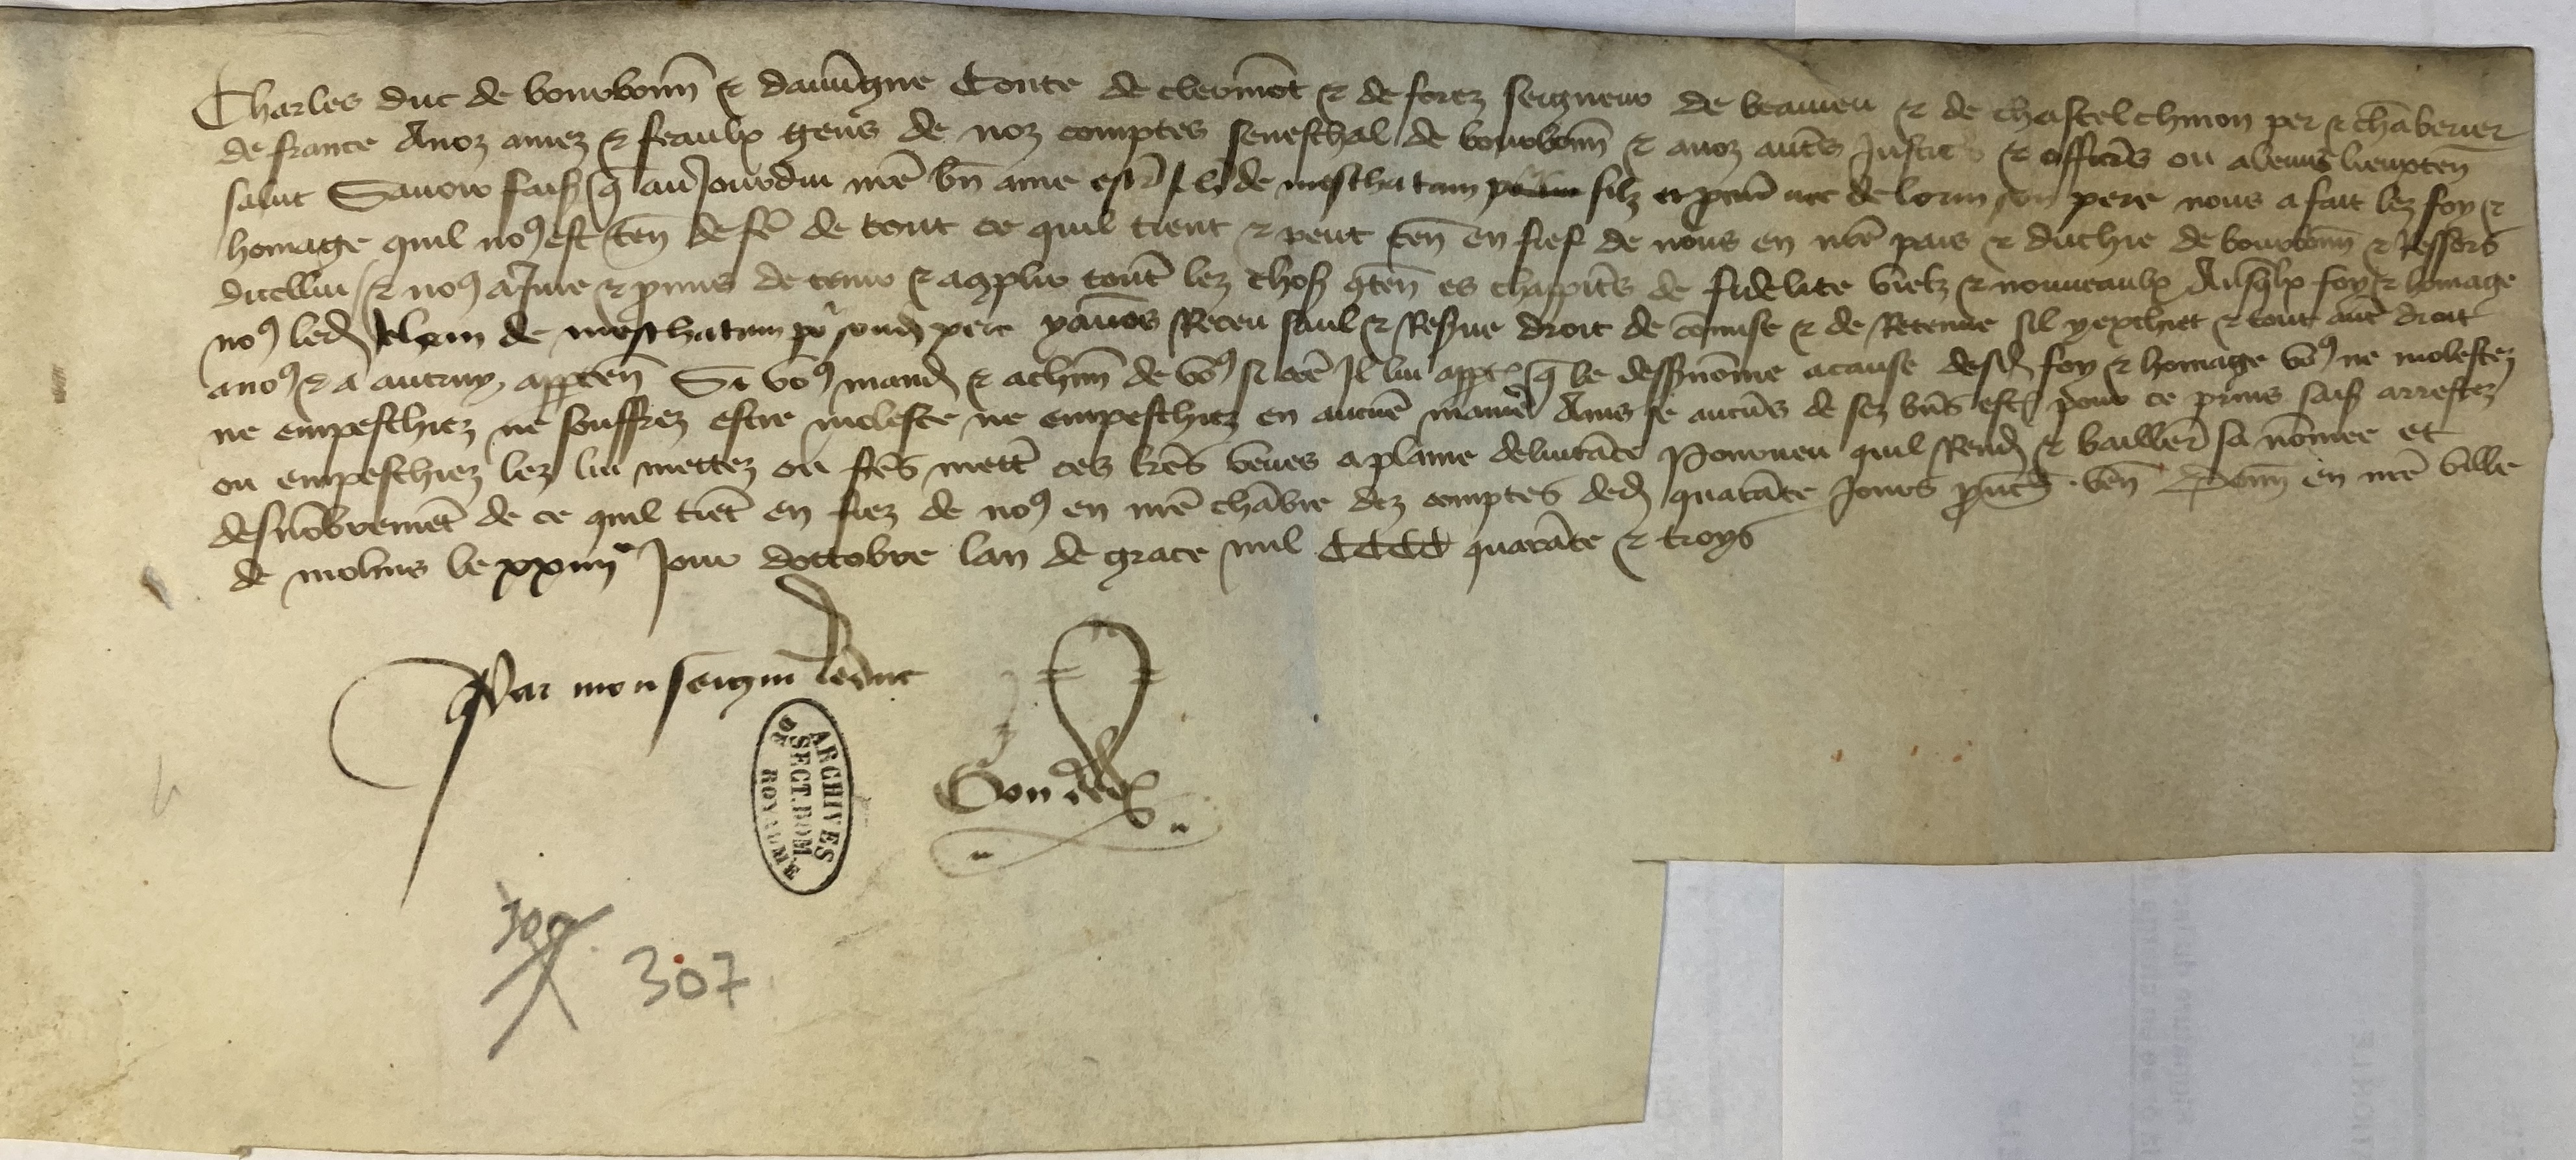
\includegraphics[scale=0.115]{front/images/1443_10_24b.jpg}
    \caption{Photographie de l'acte daté du 24 octobre 1443. \newline Charles, duc de Bourbonnais et d'Auvergne, etc., notifie aux gens de ses comptes qu'il a reçu l'hommage de Jean de Meschatain pour tout ce que celui-ci tient de lui en fief dans le duché de Bourbonnais.}
    \label{fig:1443_10_24b}
\end{figure} 

\par À partir des photographies prises, les actes sont transcrits selon les normes développées dans les \textit{Conseils pour l'édition des textes médiévaux}\footnote{\cite{guyotjeanninConseilsPourEdition2009}.}. La transcription donne accès au contenu du texte et à des informations essentielles comme la datation, le lieu de rédaction, ou encore des noms d'individus, qui vont permettre de compléter le schéma XML. La deuxième étape consiste à encoder l'acte. La transcription peut avoir lieu directement à cette étape si le texte n'est pas trop difficile à lire\footnote{Encodage des actes concernés : Gitlab \newline (xml/bourbon/charles\_i\_bourbon/brb\_ch\_i\_1443\_10\_24a.xml), \newline (xml/bourbon/charles\_i\_bourbon/brb\_ch\_i\_1443\_10\_24b.xml), \newline (xml/bourbon/charles\_i\_bourbon/brb\_ch\_i\_1443\_10\_24c.xml), \newline (xml/bourbon/charles\_i\_bourbon/brb\_ch\_i\_1443\_10\_25a.xml), \newline (xml/bourbon/charles\_i\_bourbon/brb\_ch\_i\_1454\_10\_22a.xml).}. Le TEI Header est complété avec des informations d'identification de l'acte. La date est nécessaire pour remplir l'attribut \og xml:id \fg \space de la balise <TEI> ainsi que le titre de niveau \og a \fg. Ensuite, c'est tout le contenu de la balise <sourceDesc>, décrivant le document, soit l'acte concerné, qui est à remplir avec les identifiants de l'acte : institution de conservation, fonds, cote ainsi que sa date de rédaction. Puis, viennent la liste des personnes mentionnées : prince à l'origine de l'acte et signataire. Enfin, le <sourceDesc> est complété par le tableau de la tradition. Le <profileDesc> contient les informations contextuelles, soit un résumé en quelques mots de l'acte en question. 
\newpage

\par Une fois le TEI Header complété, c'est le <text> avec les attributs de la première <div> : identifiants, état, type diplomatique. Les balises enfant de la balise <docDate> sont enrichies des dates de temps et de lieu. Ensuite, l'analyse précède le texte transcrit. Le texte de l'acte est retranscrit tel quel et les lettres et les graphies manquantes ou erronées sont déclarées au sein de l'apparat critique. Des balises signalent les personnes et les lieux du texte. Ces deux derniers éléments, ainsi que le signataire, qui clôt le texte, sont référencés. 
\newline 

\begin{figure}[H]
    \centering
    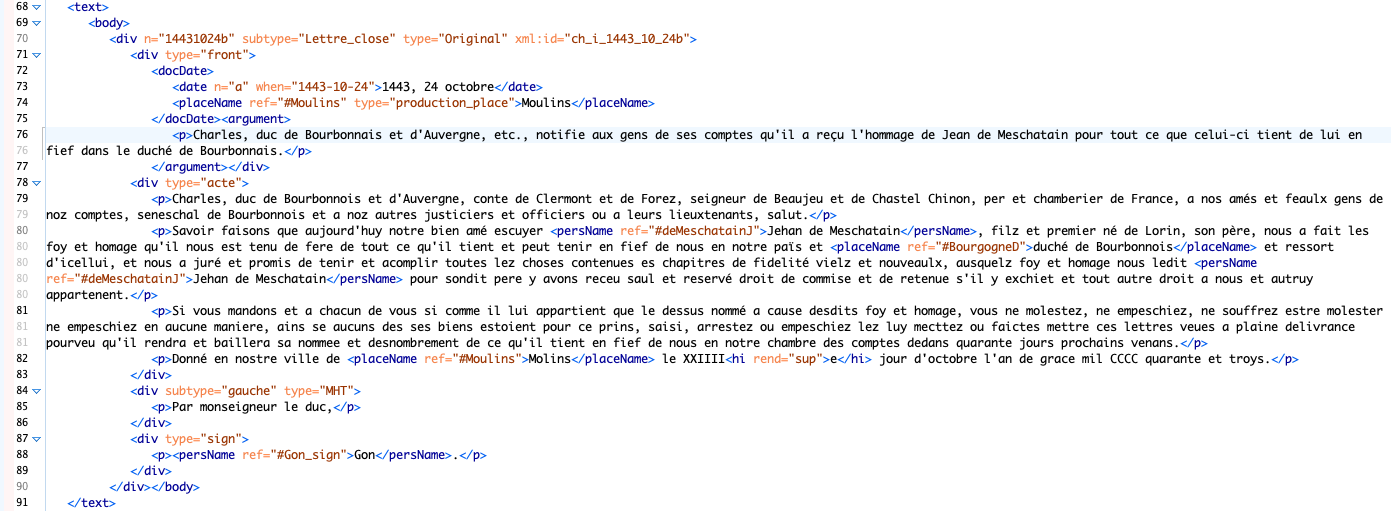
\includegraphics[scale=0.33]{front/images/encodage_text.png}
    \caption{Encodage TEI du texte de l'acte daté du 24 octobre 1443.}
    \label{fig:encodage_1443}
\end{figure} 

\par Toutes les étapes préalables à la mise en ligne des données détaillées dans les sections précédentes sont réplicables, ce qui rend possible l'élargissement du corpus lorsque de nouveaux actes de même nature sont découverts. En effet, il est possible de relancer les scripts afin d'assurer la transformation en LaTeX et la compilation en PDF du corpus, une fois les nouveaux actes encodés en XML, et ainsi les ajouter aux éléments déjà mis en ligne. Toutefois, ce procédé fonctionne et représente un gain de temps pour des corpus édités sur du traitement de texte et dont les inédits ne sont pas trop nombreux à ajouter. Afin de traiter des corpus qui n'auraient pas été édités, il serait plus pertinent de fragmenter le texte des actes et les informations le concernant, nécessaires à l'élaboration d'une édition, pour les intégrer à une base de données, qui, parsée par un script Python, pourrait permettre de générer un encodage en XML\footnote{Cette méthode est développé dans : \cite{devaleriolaOrdinateurAuService2020}.}. 

\newpage
\thispagestyle{empty}
\mbox{}
\newpage